\documentclass[11pt]{article}

\usepackage[review]{acl}

\usepackage{times}
\usepackage{latexsym}
\usepackage[T1]{fontenc}
\usepackage[utf8]{inputenc}
\usepackage{microtype}
\usepackage{inconsolata}
\usepackage{graphicx}
\usepackage{amsmath}
\usepackage{amssymb}
\usepackage{booktabs}
\usepackage{tipa}
\usepackage{CJKutf8}
\usepackage{tikz}
\usetikzlibrary{arrows.meta, positioning, shapes.geometric}

\title{Singable Lyrics Translation with IPA-Augmented LLM Agents}

\author{Anonymous}

\begin{document}
\maketitle

\begin{abstract}
Translating song lyrics while preserving singability requires satisfying musical constraints, including syllable counts, rhyme schemes, and syllable patterns, that standard machine translation ignores.
We present a framework that exposes IPA-based phonetic analysis as a suite of composable Agent Skills, each defined by a natural-language description plus deterministic verification scripts that the orchestrating LLM invokes on demand.
The agent extracts constraints from source lyrics, then translates through a multi-phase process, calling skills to iteratively verify and refine each constraint.
We formalize the three musical constraints, describe the IPA skill suite and agent architecture, and propose three evaluation metrics: Syllable Error Rate (SER), Syllable Count Relative Error (SCRE), and Adjusted Rand Index (ARI).
A phase ablation study confirms that iterative tool-verified refinement dramatically improves constraint satisfaction and preserves rhyme structure substantially better than a supervised baseline, while requiring no task-specific training, no parallel corpora, and generalizing to any of the 100+ languages supported by eSpeak-NG.
\end{abstract}

\section{Introduction}

A translated song lyric must conform to the musical structure of the original so that it remains \emph{singable} to the same melody \citep{low-2005-pentathlon}.
This requires satisfying hard structural constraints: syllable counts must match melodic phrases, rhyme schemes should be preserved, and word-level syllable distributions should mirror the original phrasing.
Despite theoretical grounding \citep{low-2005-pentathlon,franzon-2008-choices}, computational approaches remain scarce.
Neural MT systems have no mechanism for phonetic constraints, and constrained decoding methods \citep{hokamp-liu-2017-lexically,post-vilar-2018-fast} address lexical but not phonetic constraints.
A fundamental obstacle is that \emph{counting syllables, detecting rhyme, and analyzing phonetic patterns are not tasks that LLMs perform reliably through text generation alone} \citep{gao-etal-2023-pal}.

We address this by exposing IPA-based phonetic analysis as a suite of Agent Skills, where each capability is packaged as a directory of natural-language instructions plus deterministic scripts that the orchestrating LLM discovers and invokes during translation \citep{yao-etal-2023-react}.
Unlike supervised approaches, the framework requires no parallel lyric corpora, supports any language pair via eSpeak-NG, and scales with LLM capability.
Our framework is open-source for reproducibility and practical use.\footnote{Code and Skills available at \url{https://github.com/anonymous} (anonymized for review).}

Our contributions are:
\begin{enumerate}
    \item A formalization of three musical constraints (syllable counts, rhyme schemes, and syllable patterns) and IPA-based methods for their extraction and verification (\S\ref{sec:constraints}).
    \item An IPA-augmented Skill suite and multi-phase orchestration architecture for constraint-preserving lyrics translation (\S\ref{sec:framework}).
    \item Three automatic evaluation metrics (SER, SCRE, and ARI) designed to measure structural constraint preservation in singable translation (\S\ref{sec:eval}).
\end{enumerate}
To our knowledge, this is the first framework to package IPA-based phonetic analysis as Agent Skills for singable lyrics translation.

\section{Related Work}

\subsection{Song Translation}

Theoretical accounts treat song translation as balancing singability, sense, naturalness, rhythm, and rhyme \citep{low-2005-pentathlon,franzon-2008-choices,low-2022-translating}.
Computationally, prior work has formalized singable lyric translation as constrained sequence-to-sequence learning \citep{ou-etal-2023-songs}, addressed tonal-language constraints \citep{guo-etal-2022-automatic}, applied constrained decoding to neural poetry \citep{ghazvininejad-etal-2018-neural}, modeled musical features during generation \citep{ye-etal-2024-sing}, and used curriculum reinforcement learning \citep{ren-etal-2025-lyricar}.
Related directions include melody-constrained lyric editing \citep{zhao-etal-2025-reffly}, structural constraints in melody-to-lyric generation \citep{ou-etal-2023-loaf}, multilingual datasets and evaluation \citep{cho-etal-2025-mavl,kim-etal-2023-computational,kim-etal-2024-kpop}, scansion-based and prosody-aware lyric generation \citep{chen-teufel-2024-scansion,liang-etal-2024-xai,yu-etal-2025-songglm}, and multimodal singability \citep{yoo-etal-2025-elmi}.
These approaches rely on specialized fine-tuning, constrained decoding, or reinforcement learning; our work instead augments a general-purpose LLM with IPA verification skills, requiring no task-specific training.

\subsection{Constrained Text Generation}

Lexically constrained decoding has been studied via Grid Beam Search and Dynamic Beam Allocation \citep{hokamp-liu-2017-lexically,post-vilar-2018-fast}, while computational poetry has used finite-state machinery and neural models for meter and rhyme \citep{ghazvininejad-etal-2016-generating,hopkins-kiela-2017-automatically,lau-etal-2018-deep}.
These methods enforce constraints at the decoding level or learn them implicitly; ours lets the LLM generate freely and verifies via external phonetic skills.

\subsection{Tool-Augmented Language Models}

Prior work has shown that LLMs can be trained or prompted to invoke external tools \citep{schick-etal-2023-toolformer}, interleave reasoning with tool calls \citep{yao-etal-2023-react}, and offload computation to program execution \citep{gao-etal-2023-pal}, the latter directly relevant here since syllable counting is unreliable in text generation but deterministic via IPA tools.
Chain-of-thought prompting \citep{wei-etal-2022-chain} provides complementary structured reasoning that we combine with skill-decomposed tool use.
More recently, frontier LLM platforms have introduced \emph{Agent Skills}: capabilities packaged as a directory containing a natural-language description (\texttt{SKILL.md}) plus optional helper scripts that the orchestrating model loads on demand; we adopt this design to factor phonetic analysis into independent, reusable skills.
In machine translation, \citet{jiao-etal-2023-chatgpt} showed LLMs achieve strong translation quality, but did not consider musical or structural constraints.

\subsection{Phonetic Resources}

Our skill suite builds on Phonemizer \citep{bernard-titeux-2021-phonemizer} for text-to-IPA conversion and PanPhon \citep{mortensen-etal-2016-panphon} for phonetic distance computation; both are described in \S\ref{sec:framework}.
Concurrently, \citet{chen-etal-2025-ipa-translation} explored using IPA as an intermediary representation for LLM-based translation of spoken-only languages; while their focus is on low-resource language preservation rather than musical constraints, both approaches share the insight that IPA provides a language-agnostic phonetic interface for LLMs.

\section{Musical Constraints in Lyrics Translation}
\label{sec:constraints}

A singable translation must satisfy three structural constraints, each arising from a different aspect of the relationship between lyrics and melody.

\subsection{Syllable Count Constraint}
\label{sec:syllable-count}

In sung performance, each syllable maps to one or more musical notes.
When a melody assigns three notes to a phrase, the lyric must contain exactly three syllables; fewer leave notes unmatched, while extra syllables force cramming that disrupts the rhythmic feel.
This makes syllable count the most rigid of the three constraints: rhyme and phrasing mismatches may be tolerable in some styles, but syllable count mismatches are almost always audible.
Formally, given source lyrics $L_s = (l_1, \ldots, l_n)$ in language $\lambda_s$, the constraint requires that translated lyrics $L_t = (l'_1, \ldots, l'_n)$ in target language $\lambda_t$ satisfy $\text{syll}(l'_i, \lambda_t) = \text{syll}(l_i, \lambda_s)$ for all lines $i$.

Syllable counting is language-dependent.
For Chinese, each character constitutes exactly one syllable, so counting is trivial.
For other languages, we convert text to IPA via Phonemizer \citep{bernard-titeux-2021-phonemizer} and count \emph{vowel nuclei}, the vocalic centers of syllables:
\begin{equation}
    \text{syll}(l_i, \lambda_s) = \big|\text{nuclei}\big(\text{IPA}(l_i, \lambda_s)\big)\big|
    \label{eq:syllcount}
\end{equation}
where $\text{nuclei}(\cdot)$ matches a predefined set of IPA vowel symbols and diphthongs (e.g., \textipa{a, i, u, @, aI, eI, oU}), with adjacent vowels forming diphthongs counted as single nuclei.
For example, ``\emph{Let it go}'' yields IPA /\textipa{lEt It g@U}/ with three vowel nuclei [\textipa{E}, \textipa{I}, \textipa{@U}], giving a count of 3.
The resulting sequence $\mathbf{s} = (s_1, \ldots, s_n)$ serves as the hard constraint for translation.

\subsection{Rhyme Scheme Constraint}
\label{sec:rhyme-scheme}

Rhyme provides structural cohesion in lyrics, creating sonic expectations that are satisfying when met and jarring when violated.
A song with an $AABB$ scheme feels fundamentally different from one with $ABAB$; preserving the rhyme scheme ensures the translation maintains the same pattern of sonic echoes as the original.
Formally, a rhyme scheme is a labeling $R = (r_1, \ldots, r_n)$ where $r_i \in \{A, B, C, \ldots\}$ assigns each line to a rhyme class, with $r_i = r_j$ if and only if lines $i$ and $j$ rhyme.
The constraint requires that the translation's scheme $R_t$ match the source scheme $R_s$.

We detect rhyme by comparing phonetic endings rather than orthographic forms.
For each line, we extract the \emph{rhyme ending}: the IPA substring from the last vowel nucleus to the end of the transcription.
For Chinese, we extract the pinyin final of the last character instead.
The scheme is constructed by labeling the first line $A$, and assigning each subsequent line the label of any earlier line it rhymes with, or a new label otherwise.
Consider the following example:
\begin{quote}
\small
\emph{The stars shine bright with silver \textbf{light}} $\rightarrow$ /\textipa{laIt}/ $\rightarrow$ ending: /\textipa{aIt}/ \\
\emph{And covers all in purest \textbf{white}} $\rightarrow$ /\textipa{waIt}/ $\rightarrow$ ending: /\textipa{aIt}/ \\
\emph{I stand and watch the world \textbf{below}} $\rightarrow$ /\textipa{bIl@U}/ $\rightarrow$ ending: /\textipa{@U}/ \\
\emph{As gentle winds begin to \textbf{blow}} $\rightarrow$ /\textipa{bl@U}/ $\rightarrow$ ending: /\textipa{@U}/
\end{quote}
Lines 1--2 share ending /\textipa{aIt}/ (class $A$) and lines 3--4 share /\textipa{@U}/ (class $B$), yielding $AABB$.
This IPA-based approach correctly identifies rhymes that orthographic comparison would miss (e.g., ``weight'' and ``late'') and rejects false rhymes based on spelling alone (e.g., ``cough'' and ``through'').

\subsection{Syllable Pattern Constraint}
\label{sec:syllable-pattern}

Even when two lines share the same total syllable count, different word-level distributions create different rhythmic feels.
Consider two eight-syllable lines: ``un-for-get-ta-ble mel-o-dy'' with pattern $[5, 3]$ versus ``I can hear the mu-sic play'' with pattern $[1, 1, 1, 1, 2, 2]$.
The first has two long words producing a flowing feel, while the second has many short words producing a staccato rhythm.
Word boundaries interact with note groupings and breaths in sung performance, so preserving the syllable pattern ensures the translation fits the melody at the phrasing level, not just the syllable level.
Formally, the syllable pattern of a line $l_i$ is a vector $\mathbf{p}_i = (p_{i,1}, \ldots, p_{i,k_i})$ recording the syllable count of each word. The constraint asks that the translation's pattern $\mathbf{p}'_i$ be similar to $\mathbf{p}_i$ while maintaining the same total: $\sum_j p'_{i,j} = \sum_j p_{i,j} = s_i$.

To extract patterns, we apply language-specific word segmentation (space-based tokenization for English and other space-delimited languages, and a neural tokenizer for Chinese), then compute each word's syllable count via Equation~\ref{eq:syllcount}.
We measure pattern similarity using a normalized alignment score.
Given patterns of potentially different lengths, we pad the shorter one with zeros and compute:
\begin{equation}
    \text{sim}(\mathbf{p}, \mathbf{p}') = 1 - \frac{\sum_{j=1}^{m} |p_j - p'_j|}{\sum_{j=1}^{m} \max(p_j, p'_j)}
    \label{eq:patsim}
\end{equation}
where $m = \max(|\mathbf{p}|, |\mathbf{p}'|)$.
A score of 1.0 indicates an exact match; we treat $\geq 0.8$ as acceptable.
For example, ``Let it go'' has pattern $[1, 1, 1]$.
A Chinese translation tokenized as two words with pattern $[2, 1]$ yields $\text{sim}([1,1,1], [2,1,0]) = 0.5$ (poor alignment), whereas a translation tokenized as three single-character words gives pattern $[1, 1, 1]$ with $\text{sim} = 1.0$.

\section{IPA-Augmented Skill Framework}
\label{sec:framework}

Figure~\ref{fig:framework} overviews the skill orchestration architecture.

\begin{figure}[t]
\centering
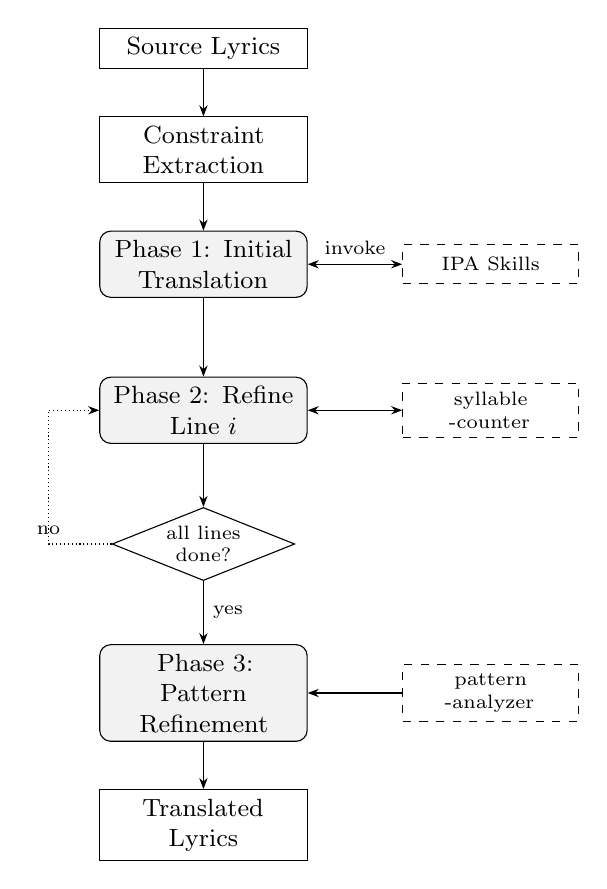
\begin{tikzpicture}[
    node distance=0.6cm and 1.0cm,
    every node/.style={font=\small},
    box/.style={rectangle, draw, text width=2.4cm, minimum height=0.5cm, align=center},
    phase/.style={rectangle, draw, rounded corners, fill=gray!10, text width=2.4cm, minimum height=0.5cm, align=center},
    tool/.style={rectangle, draw, dashed, fill=white, text width=2.0cm, minimum height=0.5cm, align=center, font=\scriptsize},
    check/.style={diamond, draw, aspect=2.5, inner sep=1pt, font=\scriptsize, align=center},
    >={Stealth[length=4pt]},
]
% Main flow
\node[box] (src) {Source Lyrics};
\node[box, below=of src] (ext) {Constraint\\Extraction};
\node[phase, below=of ext] (p1) {Phase 1: Initial\\Translation};
\node[tool, right=1.2cm of p1] (t1) {IPA Skills};
\node[phase, below=1.0cm of p1] (p2) {Phase 2: Refine\\Line $i$};
\node[tool, right=1.2cm of p2] (t2) {syllable\\-counter};
\node[check, below=0.8cm of p2] (c2) {all lines\\done?};
\node[phase, below=0.8cm of c2] (p3) {Phase 3: Pattern\\Refinement};
\node[tool, right=1.2cm of p3] (t3) {pattern\\-analyzer};
\node[box, below=of p3] (out) {Translated Lyrics};

% Vertical flow
\draw[->] (src) -- (ext);
\draw[->] (ext) -- (p1);
\draw[->] (p1) -- (p2);
\draw[->] (p2) -- (c2);
\draw[->] (c2) -- node[right, font=\scriptsize] {yes} (p3);
\draw[->] (p3) -- (out);

% Skill interactions: bidirectional invocation for Phases 1--2, one-way analysis for Phase 3
\draw[<->] (p1) -- node[above, font=\scriptsize] {invoke} (t1);
\draw[<->] (p2) -- (t2);
\draw[<-] (p3) -- (t3);

% Phase 2 graph-level loop (per-line iteration)
\draw[->, densely dotted] (c2.west) -- ++(-0.8,0) node[above, font=\scriptsize] {no} |- (p2.west);

\end{tikzpicture}
\caption{Skill framework overview. Phase~1 translates all lines using an internal tool-use loop that invokes the IPA skills. Phase~2 refines each line sequentially (up to 10 attempts per line); the dotted arrow shows the orchestration loop that iterates through lines. Phase~3 is a single pass that uses the \texttt{syllable-pattern-analyzer} skill output to guide pattern refinement without a retry loop.}
\label{fig:framework}
\end{figure}

\subsection{IPA as Universal Phonetic Interface}

The International Phonetic Alphabet provides a standardized, language-independent representation of speech sounds, making it an ideal intermediary for cross-lingual phonetic analysis: regardless of the source or target language, all phonetic operations (syllable counting, rhyme comparison, pattern analysis) can be performed on IPA transcriptions using the same algorithms.
Our system uses Phonemizer \citep{bernard-titeux-2021-phonemizer} as the text-to-IPA backend, wrapping the eSpeak~NG speech synthesizer with support for over 100 languages.
Language codes are normalized internally (e.g., \texttt{zh}, \texttt{zh-cn}, \texttt{cmn} all map to Mandarin Chinese) to provide a uniform interface.
For phonetic distance computation, we use PanPhon \citep{mortensen-etal-2016-panphon}, which maps each IPA segment to a vector of articulatory features, enabling fine-grained similarity measurement.

\subsection{Skill Suite}
\label{sec:tools}

The orchestrator has access to a suite of Agent Skills (Table~\ref{tab:tools}), each packaged as a \texttt{SKILL.md} description plus a deterministic verification script.
The four IPA-based analytic skills (\texttt{syllable-counter}, \texttt{phonetic-analyzer}, \texttt{rhyme-analyzer}, \texttt{syllable-pattern-analyzer}) wrap functions that provide capabilities the LLM cannot reliably perform through text generation alone \citep{gao-etal-2023-pal}; \texttt{lyrics-validator} and \texttt{lyrics-translator} sit on top to compose them.

\begin{table}[t]
\centering
\small
\begin{tabular}{@{}p{3.0cm}p{4.2cm}@{}}
\toprule
\textbf{Skill} & \textbf{Description} \\
\midrule
\texttt{syllable-counter} & Count syllables via IPA vowel nuclei (or character count for Chinese) \\
\texttt{phonetic-analyzer} & Convert text to IPA via eSpeak~NG and compute phonetic similarity \\
\texttt{rhyme-analyzer} & Detect the rhyme scheme by comparing IPA endings \\
\texttt{syllable-pattern-\allowbreak{}analyzer} & Compare target vs.\ current syllable patterns with structured feedback \\
\texttt{lyrics-validator} & Validate all three constraints jointly on a translated line set \\
\texttt{lyrics-translator} & Top-level orchestration skill coordinating the five sub-skills above through the multi-phase loop in \S\ref{sec:loop} \\
\bottomrule
\end{tabular}
\caption{Agent Skills exposed to the orchestrating LLM. Each skill is a directory with a \texttt{SKILL.md} description plus deterministic verification scripts; all skills accept a language parameter for language-specific processing.}
\label{tab:tools}
\end{table}

The \texttt{syllable-counter} skill is the most frequently invoked: given a text string and language code, it converts to IPA and returns an integer syllable count (\S\ref{sec:syllable-count}).
The \texttt{phonetic-analyzer} skill exposes the raw IPA transcription, allowing the orchestrator to inspect phonetic realizations and reason about which syllables to modify, a form of chain-of-thought reasoning \citep{wei-etal-2022-chain} grounded in phonetic observation.
The \texttt{rhyme-analyzer} skill analyzes the IPA endings of a set of lines and returns the rhyme scheme (e.g., ``$AABB$''), ensuring judgments are phonetic rather than orthographic.
The \texttt{syllable-pattern-analyzer} skill compares a target syllable pattern against the current one, returning the similarity score (Equation~\ref{eq:patsim}), per-word differences, and natural-language suggestions for improvement.
All skills are discovered by the orchestrating LLM through their \texttt{SKILL.md} descriptions and invoked via the host's tool-use interface.

\subsection{Constraint Extraction}
\label{sec:extraction}

Before translation begins, the system extracts all three constraints from the source lyrics $L_s$ in language $\lambda_s$: (1) \textbf{syllable counts} $\mathbf{s} = (s_1, \ldots, s_n)$ via \texttt{syllable-counter} on each line, (2) \textbf{rhyme scheme} $R_s$ via \texttt{rhyme-analyzer} on all lines, and (3) \textbf{syllable patterns} $P_s = (\mathbf{p}_1, \ldots, \mathbf{p}_n)$ via \texttt{syllable-pattern-analyzer}.
These constraints are passed to the orchestrator as part of the translation prompt, providing explicit targets for each line.
Table~\ref{tab:constraints-example} shows an example.

\begin{table}[t]
\centering
\small
\begin{tabular}{@{}clcl@{}}
\toprule
\textbf{Line} & \textbf{Text} & \textbf{Syll.} & \textbf{Pattern} \\
\midrule
1 & The snow glows white & 4 & {[1,1,1,1]} \\
2 & On the mountain tonight & 6 & {[1,1,2,2]} \\
3 & Not a footprint to be seen & 7 & {[1,1,2,1,1,1]} \\
4 & A kingdom of isolation & 8 & {[1,2,1,4]} \\
\midrule
\multicolumn{4}{@{}l}{\textbf{Rhyme scheme:} $AABC$ (\emph{white}/\emph{tonight} rhyme via} \\
\multicolumn{4}{@{}l}{\quad shared IPA ending /\textipa{aIt}/; lines 3--4 are unmatched)} \\
\bottomrule
\end{tabular}
\caption{Example constraint extraction from English source lyrics. Syllable counts are computed via IPA vowel nuclei; patterns via space-based word segmentation.}
\label{tab:constraints-example}
\end{table}

\subsection{Multi-Phase Skill Orchestration}
\label{sec:loop}

Translation proceeds through three phases, encoded as procedural instructions in the top-level \texttt{lyrics-translator} \texttt{SKILL.md} that the orchestrating LLM follows, invoking the sub-skills at each step.
The design reflects the priority ordering identified by \citet{low-2005-pentathlon}: semantic content and rhythm (syllable counts) take precedence, followed by phrasing (patterns), with rhyme considered throughout but given lower priority.

\paragraph{Phase 1: Initial Translation with Skill-Guided Reasoning.}
The orchestrator receives the source lyrics, target language, and all extracted constraints from the \texttt{lyrics-translator} skill instructions.
It generates an initial translation of all lines, interleaving reasoning, skill invocations to verify output, and adjustments within the same generation turn (a tool-use pattern in the spirit of \citet{yao-etal-2023-react}).
The skill instructions direct the orchestrator to consider all three constraints simultaneously, producing a ``best-effort'' initial translation.

A typical interaction proceeds as: the orchestrator reasons about the target syllable count for a line, drafts a translation, invokes \texttt{syllable-counter} to verify, observes the result, and adjusts if needed, continuing until all lines are translated.

\paragraph{Phase 2: Line-by-Line Syllable Refinement.}
The initial translation rarely satisfies all syllable constraints exactly.
In this phase, the orchestrator processes each line individually, invoking \texttt{syllable-counter} and comparing the result to the target.
If there is a mismatch, the skill returns explicit feedback (e.g., ``Line $i$ has $s'_i$ syllables but the target is $s_i$; please revise while preserving meaning'') and the orchestrator generates a revised translation.
The skill is re-invoked, continuing for up to 10 iterations; if no exact match is found, the closest attempt is retained.
This phase is critical because even a single syllable mismatch can make a line unsingable.

\paragraph{Phase 3: Syllable Pattern Refinement.}
After syllable counts are matched, the orchestrator refines word-level syllable distributions.
For each line, \texttt{syllable-pattern-analyzer} compares the current pattern against the target and returns structured feedback including the similarity score, per-word differences, and suggestions (e.g., ``split the first word into shorter components'').
For each mismatched line, the orchestrator generates a revised translation; the revision is accepted only if it improves pattern similarity while maintaining the correct total syllable count, and is otherwise reverted.
Lines whose patterns already match the target are left unchanged.

\paragraph{Priority and termination.}
The three-phase design addresses constraints in order of importance: syllable counts first (hardest constraint), then syllable patterns.
Rhyme is monitored throughout Phases 1 and 2 via \texttt{rhyme-analyzer}, but is not given a dedicated refinement phase because rhyme violations are generally less disruptive to singability than syllable mismatches \citep{low-2005-pentathlon}.
The process terminates after Phase 3 with a final \texttt{lyrics-validator} pass.

\subsection{Worked Example}

To illustrate, consider translating ``\emph{Not a footprint to be seen}'' (7 syllables, pattern $[1, 1, 2, 1, 1, 1]$) into Chinese.
In Phase~1, the orchestrator produces a 7-character translation; syllable counting confirms the match, so Phase~2 skips this line.
In Phase~3, pattern analysis reveals the Chinese tokenization yields $[3, 2, 2]$ with similarity 0.38 against the target, and suggests splitting the first word.
The orchestrator revises to a translation with single-character tokenization, yielding $[1, 1, 1, 1, 1, 1, 1]$ and similarity 0.71: an improvement, though not exact.
This illustrates a fundamental challenge: Chinese word boundaries are determined by semantics and do not always permit arbitrary decomposition.

\section{Evaluation Metrics}
\label{sec:eval}

Standard MT metrics such as BLEU measure n-gram overlap and do not capture whether a translation preserves musical structure.
\citet{kim-etal-2023-computational} proposed a computational evaluation framework for singable lyric translation; building on this direction, we propose three complementary metrics, each targeting one of the three musical constraints.

\subsection{Syllable Error Rate (SER)}

SER measures the overall alignment between the source and translated syllable count sequences using the Levenshtein edit distance \citep{levenshtein-1966}:
\begin{equation}
    \text{SER} = \frac{\text{Lev}(\mathbf{s}, \mathbf{s}')}{\max(|\mathbf{s}|, |\mathbf{s}'|)}
\end{equation}
where $\mathbf{s} = (s_1, \ldots, s_n)$ and $\mathbf{s}' = (s'_1, \ldots, s'_m)$ are the source and translated syllable count sequences, and $\text{Lev}$ operates over sequences of integers (with substitution cost equal to 1 regardless of the magnitude of the difference).

SER captures both \emph{substitution errors} (a line has the wrong syllable count) and \emph{structural errors} (lines are missing or added).
$\text{SER} = 0$ indicates perfect preservation; higher values indicate greater divergence.
Unlike per-line metrics, SER penalizes translations that drop or add lines, which is important because line structure directly corresponds to melodic phrases.

\subsection{Syllable Count Relative Error (SCRE)}

SCRE provides a normalized, per-line view of syllable accuracy, assuming the translation preserves the number of lines ($m = n$):
\begin{equation}
    \text{SCRE} = \frac{1}{n} \sum_{i=1}^{n} \frac{|s_i - s'_i|}{s_i}
\end{equation}

SCRE weights errors relative to line length: a two-syllable error on a four-syllable line ($\text{SCRE}_i = 0.5$) is penalized more heavily than on a twelve-syllable line ($\text{SCRE}_i = 0.17$).
This reflects the intuition that short lines leave less room for syllabic deviation; a single extra syllable in a three-syllable phrase is far more noticeable than in a long verse.
$\text{SCRE} = 0$ indicates all lines match exactly.

SER and SCRE are complementary: SER captures structural alignment including line count mismatches, while SCRE provides percentage-based accuracy that is more interpretable for line-by-line comparison.

\subsection{Adjusted Rand Index (ARI)}

To measure rhyme scheme preservation, we treat the rhyme scheme as a \emph{clustering} of lines and compute the Adjusted Rand Index \citep{hubert-arabie-1985} between the source and translated clusterings.

Let $R_s = (r_1, \ldots, r_n)$ and $R_t = (r'_1, \ldots, r'_n)$ be the rhyme scheme labelings.
The Rand Index (RI) counts the fraction of line pairs that are either in the same cluster in both schemes or in different clusters in both schemes.
ARI adjusts RI for the expected value under random label assignments:
\begin{equation}
    \text{ARI} = \frac{\text{RI} - \mathbb{E}[\text{RI}]}{\max(\text{RI}) - \mathbb{E}[\text{RI}]}
\end{equation}

ARI $\in [-1, 1]$: $1$ indicates the translation perfectly preserves the rhyme structure, $0$ indicates chance-level agreement, and negative values indicate systematic disagreement.
Crucially, ARI is robust to label permutation: a source with scheme $AABB$ and a translation with $BBAA$ receives $\text{ARI} = 1$, since the grouping structure is identical.

Together, SER, SCRE, and ARI cover the structural dimensions of singable translation.
They do not measure semantic fidelity or naturalness and are complementary to standard MT metrics such as BLEU and COMET.

\section{Experiments}
\label{sec:experiments}

\subsection{Setup}

We evaluate on English-to-Chinese ($\text{en} \rightarrow \text{cmn}$) song translation using 100 test cases (5 lines each) from the publicly available test split of the parallel lyric corpus released by \citet{ou-etal-2023-songs}.\footnote{\url{https://huggingface.co/datasets/LongshenOu/lyric-trans-en2zh-data}}
The dataset covers pop, ballad, rock, and musical-theatre genres.
Our open-source release (Apache-2.0) ships the full Skill suite (six \texttt{SKILL.md} directories with their verification scripts), the IPA tool implementations, and evaluation scripts under the \texttt{blt-skills} repository, enabling reproduction on any user-supplied lyrics in any language pair supported by eSpeak-NG.

\paragraph{Implementation.}
The framework is implemented as Agent Skills: each phase is encoded as procedural instructions in the orchestrating \texttt{lyrics-translator} \texttt{SKILL.md}, which references the five sub-skills (\S\ref{sec:tools}) and invokes their verification scripts as needed.
For LLM inference, we evaluate Qwen3-30B (4-bit quantized) served locally via Ollama as a representative open-weight orchestrator.
The same Skill suite is directly compatible with frontier models that support the Agent Skills interface (e.g., Claude via Claude Code), and supplementary Claude-orchestrated runs are reported in our open-source benchmark scripts.\footnote{See \texttt{scripts/run\_cc.py} and \texttt{scripts/run\_bench.py} in the released code.}
The IPA verification scripts are exposed to the orchestrator through each skill's \texttt{SKILL.md} description.

\paragraph{Conditions.}
We conduct a phase ablation study alongside a supervised baseline:
\begin{itemize}
    \item \textbf{Phase~1 only}: Initial translation with IPA skill access but no iterative refinement.
    \item \textbf{Phase~1+2}: Adds line-by-line syllable count refinement (up to 10 iterations per line).
    \item \textbf{Phase~1+2+3} (full BLT Skills): Adds syllable pattern refinement after syllable counts are matched.
    \item \textbf{CLT} \citep{ou-etal-2023-songs}: A supervised mBART model fine-tuned with explicit length, rhyme, and word-boundary constraint tokens. This represents a task-specific training approach and serves as an upper bound for constraint satisfaction.
\end{itemize}
All BLT conditions use the same Qwen3-30B orchestrator and the same Skill suite; CLT uses its own fine-tuned checkpoint.
We report SER, SCRE, and ARI as defined in \S\ref{sec:eval}.

\subsection{Results and Phase Ablation}

Table~\ref{tab:ablation} presents the results of the phase ablation study.

\begin{table}[t]
\centering
\small
\begin{tabular}{@{}lccc@{}}
\toprule
\textbf{Method} & \textbf{SER} $\downarrow$ & \textbf{SCRE} $\downarrow$ & \textbf{ARI} $\uparrow$ \\
\midrule
Phase 1 only         & 0.8343 & 0.2076 & 0.3133 \\
Phase 1+2            & \underline{0.2151} & \underline{0.0291} & \textbf{0.3623} \\
Phase 1+2+3 (full)   & 0.3132 & 0.0457 & 0.2951 \\
\midrule
CLT \citep{ou-etal-2023-songs} & \textbf{0.0860} & \textbf{0.0142} & 0.0015 \\
\bottomrule
\end{tabular}
\caption{Phase ablation and baseline comparison ($\text{en} \rightarrow \text{cmn}$, $n{=}100$). Bold = best overall; underline = best among BLT variants.}
\label{tab:ablation}
\end{table}

\paragraph{Phase~2 is the critical stage.}
Adding syllable refinement reduces SER by 74.2\% (0.83$\to$0.22) and SCRE by 86.0\% (0.21$\to$0.03), confirming that iterative skill-verified refinement, not merely skill access during initial generation, drives constraint satisfaction.
The cost is a 4.8$\times$ increase in inference time (7.0\,s $\to$ 33.5\,s per test case on a single NVIDIA RTX~3090; timings include all phases up to and including the indicated phase).
This latency remains practical for offline lyric translation, where constraint satisfaction outweighs speed.

\paragraph{Phase~3 trades syllable accuracy for rhyme.}
Pattern refinement increases SER (+45.6\%) and SCRE (+57.0\%) because adjusting word boundaries disrupts syllable counts that Phase~2 had matched.
ARI also decreases by 18.6\% (0.36$\to$0.30), suggesting that at scale, pattern refinement is too aggressive and requires more conservative application, e.g., a higher skip threshold or explicit rhyme preservation checks.

\paragraph{Comparison with CLT.}
The supervised CLT baseline achieves strong syllable accuracy (SCRE 0.014) through explicit constraint tokens and task-specific fine-tuning.
However, its ARI is near zero (0.002), indicating that its constraint mechanism does not preserve rhyme structure.
The best BLT variant (Phase~1+2) achieves substantially higher ARI (0.36 vs.\ 0.002) while requiring no task-specific training, only IPA skills and a general-purpose LLM.
CLT is also limited to the single language pair it was trained on, whereas BLT operates on any language pair supported by Phonemizer's eSpeak-NG backend, covering over 100 languages without retraining.

\subsection{Qualitative Analysis}

Table~\ref{tab:qualitative} illustrates the pipeline on the \emph{Let It Go} excerpt from Table~\ref{tab:constraints-example}, translated from English to Chinese.
The Base LLM produces natural but unconstrained translations: line counts range from 7 to 9 characters, overshooting every target.
The BLT Skills system, guided by \texttt{syllable-counter} verification in Phase~2, matches three of four targets exactly.
Line~4 (target 8) remains one syllable short at 7; Phase~2 exhausted its 10 refinement attempts without finding an 8-character alternative that preserved meaning, retaining the closest attempt.
Phase~3 pattern refinement has limited effect here because Chinese character-level tokenization produces uniform $[1, 1, \ldots]$ patterns regardless of word grouping.

\begin{table}[t]
\centering
\small
\begin{tabular}{@{}clcc@{}}
\toprule
\textbf{Line} & \textbf{Text} & \textbf{Syll.} & \textbf{Tgt} \\
\midrule
\multicolumn{4}{@{}l}{\textbf{Source (English):}} \\
1 & The snow glows white & 4 & -- \\
2 & On the mountain tonight & 6 & -- \\
3 & Not a footprint to be seen & 7 & -- \\
4 & A kingdom of isolation & 8 & -- \\
\midrule
\multicolumn{4}{@{}l}{\textbf{Base LLM (Chinese, no tools):}} \\
1 & \begin{CJK}{UTF8}{bsmi}白雪在夜裡閃耀\end{CJK} & 7 & 4\,$\times$ \\
2 & \begin{CJK}{UTF8}{bsmi}今夜在那座山上\end{CJK} & 7 & 6\,$\times$ \\
3 & \begin{CJK}{UTF8}{bsmi}看不見任何一個腳印\end{CJK} & 9 & 7\,$\times$ \\
4 & \begin{CJK}{UTF8}{bsmi}一個與世隔絕的王國\end{CJK} & 9 & 8\,$\times$ \\
\midrule
\multicolumn{4}{@{}l}{\textbf{BLT Skills (Chinese, with IPA skills):}} \\
1 & \begin{CJK}{UTF8}{bsmi}皚皚白雪\end{CJK} & 4 & 4\,$\checkmark$ \\
2 & \begin{CJK}{UTF8}{bsmi}籠罩今夜山巔\end{CJK} & 6 & 6\,$\checkmark$ \\
3 & \begin{CJK}{UTF8}{bsmi}看不到一絲足跡\end{CJK} & 7 & 7\,$\checkmark$ \\
4 & \begin{CJK}{UTF8}{bsmi}這是孤獨的國度\end{CJK} & 7 & 8\,$\times$ \\
\bottomrule
\end{tabular}
\caption{Qualitative example: English-to-Chinese translation of the opening lines of \emph{Let It Go}. ``Syll.''\ is the actual character count; ``Tgt''\ is the source syllable count that the translation should match. BLT Skills matches 3/4 targets; the Base LLM matches 0/4.}
\label{tab:qualitative}
\end{table}

\subsection{Discussion and Future Directions}

\paragraph{Training-free versus supervised.}
The CLT comparison highlights a fundamental trade-off: supervised models achieve superior syllable accuracy but require parallel lyric corpora and per-language-pair training, whereas BLT requires no training data and natively supports any of the 100+ language pairs covered by eSpeak-NG, making it immediately applicable to low-resource pairs where no parallel lyric data exists.
Furthermore, because BLT delegates constraint satisfaction to a general-purpose LLM, its quality scales directly with model capability: as LLMs improve in reasoning and instruction-following, translation quality improves correspondingly without any retraining or architectural changes.

\paragraph{Phase~3 and the accuracy--rhyme trade-off.}
At $n{=}100$, Phase~3 degrades all three metrics, suggesting that the current pattern refinement strategy is too aggressive.
More conservative approaches, such as a higher acceptance threshold, explicit rhyme preservation checks, or applying refinement only to lines with very low pattern similarity, are natural next steps.

\paragraph{Broader evaluation.}
Our primary evaluation uses a single language pair and orchestrator (Qwen3-30B).
Extending to typologically diverse pairs, multiple model sizes, and human judgments of singability and semantic fidelity would strengthen generalizability claims.
Because the Skill suite is decoupled from any specific model and exposed through standard \texttt{SKILL.md} descriptions, swapping in stronger orchestrators (e.g., Claude, GPT-4) requires no changes to the skills or the framework itself.
The MAVL benchmark \citep{cho-etal-2025-mavl} may facilitate multilingual evaluation.

\section{Conclusion}

We have presented a framework for lyrics translation that preserves musical constraints through Agent Skills.
We formalized three musical constraints (syllable counts, rhyme schemes, and syllable patterns) and described IPA-based methods for their extraction and verification.
By packaging phonetic analysis as composable Skills and structuring translation as a multi-phase orchestration over them, our system iteratively refines translations to satisfy these constraints in priority order: syllable counts first, then patterns, with rhyme monitored throughout.
The proposed metrics (SER, SCRE, and ARI) provide automatic measurement of constraint preservation that complements standard translation quality evaluation.

A phase ablation study on English-to-Chinese translation ($n{=}100$) shows that iterative syllable refinement (Phase~2) accounts for the majority of improvement (86.0\% SCRE reduction), while comparison with a supervised baseline \citep{ou-etal-2023-songs} reveals a complementary strength: BLT Skills preserves rhyme structure (ARI 0.36 vs.\ 0.002) without task-specific training.
Unlike constrained decoding \citep{hokamp-liu-2017-lexically,post-vilar-2018-fast} or supervised approaches that require per-language-pair training, our framework is language-agnostic and scales with model capability: any LLM with Skill / tool-use support can serve as the orchestrator, the IPA skills support over 100 languages via eSpeak-NG, and advances in LLM reasoning directly improve translation quality without retraining.

Future work will focus on closing the accuracy gap with supervised methods through stronger LLMs, broader language evaluation, human judgments of singability, and integration with singing voice synthesis \citep{ren-etal-2020-deepsinger} for end-to-end singable translation.

\section*{Limitations}

Our approach has several limitations.
First, the framework's correctness depends on Phonemizer / eSpeak-NG for IPA transcription, which has uneven quality across languages; we do not provide an intrinsic evaluation of syllable-counting or rhyme-detection accuracy.
Second, Phase~3 (pattern refinement) can degrade syllable accuracy that Phase~2 achieved, and the framework lacks a dedicated rhyme refinement phase.
Third, our evaluation covers only English-to-Chinese ($n{=}100$) with a single LLM; although the framework is language-agnostic in principle, we have not validated it on other language pairs.
Fourth, the supervised CLT baseline substantially outperforms BLT on syllable metrics, indicating that the agent approach has room to improve on constraint satisfaction; the current advantage is in rhyme preservation and language-pair flexibility rather than raw accuracy.
Fifth, the multi-phase refinement loop introduces latency (34--52\,s vs.\ 0.6\,s for CLT per test case), which may limit practical deployment.
Sixth, our metrics measure structural constraint preservation but not semantic fidelity or naturalness; a complete evaluation requires human judgments.
Finally, the technical approach of invoking deterministic phonetic skills from an orchestrating LLM applies established patterns \citep{yao-etal-2023-react,gao-etal-2023-pal,schick-etal-2023-toolformer} to a new domain; the primary contribution is the formalization of musical constraints and the IPA-based Skill suite rather than a novel agent architecture.

\bibliography{custom}

\appendix

\section{Prompt Templates}
\label{app:prompts}

We provide the full prompt templates used in each phase of the multi-phase orchestration.
All prompts live inside \texttt{skills/lyrics-translator/SKILL.md} (and the phase-specific sub-skill descriptions); the orchestrating LLM loads them when the parent skill is invoked, and reads each sub-skill's \texttt{SKILL.md} when the corresponding tool is needed.

\paragraph{System prompt (all phases, from \texttt{lyrics-translator/SKILL.md}).}
\begin{quote}
\small\ttfamily
You are a lyrics translator. Translate ONE line at a time while matching the target syllable count.\\[4pt]
Available skills:\\
- syllable-counter: count syllables of a candidate translation\\
- lyrics-validator: verify a line against all three constraints\\[4pt]
WORKFLOW:\\
1. Translate the source line\\
2. Invoke syllable-counter to check your translation\\
3. If the count does not match, revise and re-check\\
4. Once correct, output the final translation with no punctuation\\[4pt]
IMPORTANT: Always verify with the skills before finalizing your answer.
\end{quote}

\paragraph{Phase~1: Initial translation.}
The orchestrator receives all source lines with their target syllable counts, the detected rhyme scheme, and the target syllable patterns.
It is instructed to translate \emph{all} lines simultaneously, invoking the relevant skills to verify constraints during generation:
\begin{quote}
\small\ttfamily
Translate ALL $N$ lines of the following lyrics to \{target\_lang\} while meeting ALL 3 musical constraints.\\[4pt]
CONSTRAINT 1: SYLLABLE COUNTS (MUST MATCH EXACTLY)\\
CONSTRAINT 2: RHYME SCHEME: \{rhyme\_scheme\}\\
CONSTRAINT 3: SYLLABLE PATTERNS: \{patterns\}\\[4pt]
Invoke the available skills to verify: (1) syllable counts match exactly, (2) rhyme scheme is correct, (3) syllable patterns are maintained.\\[4pt]
Output exactly $N$ translated lines, numbered 1--$N$.
\end{quote}

\paragraph{Phase~2: Syllable refinement.}
For each mismatched line, the orchestrator receives the current best translation and explicit corrective feedback from \texttt{syllable-counter}:
\begin{quote}
\small\ttfamily
Adjust this translation to have EXACTLY \{target\} syllables.
Focus ONLY on syllable count. Minimize meaning changes.\\[4pt]
Original: ``\{source\_line\}''\\
Current: ``\{best\_translation\}''\\
Current syllables: \{actual\}/\{target\}\\
Action: \{add/remove $k$ syllables\}\\[4pt]
STRATEGIES:\\
- If too long: remove adjectives, use shorter words, merge concepts\\
- If too short: add descriptive words, use longer characters\\[4pt]
Output ONLY the adjusted translation.
\end{quote}

\paragraph{Phase~3: Pattern refinement.}
For each line whose pattern similarity is below 0.8, the orchestrator receives a structured comparison from \texttt{syllable-pattern-analyzer}:
\begin{quote}
\small\ttfamily
Adjust the word distribution in this translation without changing total syllable count.\\[4pt]
Current pattern: \{current\} (total: $s$ syllables)\\
Target pattern: \{target\} (total: $s$ syllables)\\[4pt]
Adjustments needed: \{per-word suggestions\}\\[4pt]
Keep total syllable count at $s$. Adjust word choice to match the target pattern.\\[4pt]
Output ONLY the adjusted translation.
\end{quote}

\section{Skill Algorithms}
\label{app:tools}

We describe the core algorithms underlying each IPA skill.

\subsection{\texttt{syllable-counter}}

\begin{enumerate}
    \item Remove punctuation from input text.
    \item \textbf{Chinese:} Return the character count directly (each character = one syllable).
    \item \textbf{Other languages:} Convert text to IPA via Phonemizer / eSpeak-NG.
    \item Match all diphthong and monophthong patterns using the regex:
\end{enumerate}
\begin{quote}
\small
\texttt{DIPHTHONGS} = \textipa{aI|eI|OI|aU|oU|I@|e@|U@|aI@|aU@}\\
\texttt{VOWELS} = \textipa{[i I e E \ae{} a A 6 O o U u @ 3 2 y \o{} \oe]}\\
\texttt{PATTERN} = \texttt{DIPHTHONGS} $|$ \texttt{VOWELS}(\texttt{+combining})?
\end{quote}
\begin{enumerate}
    \setcounter{enumi}{4}
    \item Return the number of regex matches (= number of vowel nuclei = syllable count).
\end{enumerate}

\subsection{\texttt{rhyme-analyzer}}

\begin{enumerate}
    \item For each line, extract the \emph{rhyme ending}:
    \begin{itemize}
        \item \textbf{Chinese:} Use PyPinyin to extract the final (\begin{CJK}{UTF8}{bsmi}韻母\end{CJK}) of the last character.
        \item \textbf{Other languages:} Convert to IPA, find the last vowel nucleus, return the substring from that position to end-of-string.
    \end{itemize}
    \item Build the rhyme scheme by iterating through lines: assign the first line label $A$; for each subsequent line, if its ending matches any earlier line's ending (exact or substring match), assign the same label; otherwise assign the next unused label.
    \item Two lines rhyme if: \texttt{ending$_1$ == ending$_2$} $\lor$ \texttt{ending$_1$ $\subset$ ending$_2$} $\lor$ \texttt{ending$_2$ $\subset$ ending$_1$}.
\end{enumerate}

\subsection{\texttt{syllable-pattern-\allowbreak{}analyzer}}

Given target pattern $\mathbf{p}$ and current pattern $\mathbf{p}'$:
\begin{enumerate}
    \item Compute position-by-position differences for each word position $j$: $d_j = p'_j - p_j$ (zero-padded to the longer length).
    \item Compute three sub-scores:
    \begin{itemize}
        \item \emph{Position similarity} (weight 0.5): $1 - \sum_j |d_j| / \sum_j p_j$
        \item \emph{Length similarity} (weight 0.25): $1 - ||\mathbf{p}| - |\mathbf{p}'|| / \max(|\mathbf{p}|, |\mathbf{p}'|)$
        \item \emph{Total similarity} (weight 0.25): $1 - |\sum p_j - \sum p'_j| / \sum p_j$
    \end{itemize}
    \item Return the weighted sum, clipped to $[0, 1]$, along with per-word suggestions (e.g., ``word~3: has 3 syllables, target is 1'').
\end{enumerate}

Note: the similarity in the main paper (Equation~\ref{eq:patsim}) uses the simplified formulation; the implementation adds length and total sub-scores for finer-grained feedback.


\section{Hyperparameters}
\label{app:hyperparams}

Table~\ref{tab:hyperparams} lists all hyperparameters used in the experiments.

\begin{table}[h]
\centering
\small
\begin{tabular}{@{}llr@{}}
\toprule
\textbf{Category} & \textbf{Parameter} & \textbf{Value} \\
\midrule
Model & LLM & Qwen3-30B \\
Model & Quantization & Q4\_K\_M \\
Model & Temperature & 0.7 \\
\midrule
Phase~1 & Max skill invocations & 10 \\
Phase~1 & Skill set & All 6 skills \\
\midrule
Phase~2 & Max attempts / line & 10 \\
Phase~2 & Skill calls / attempt & 5 \\
\midrule
Phase~3 & Pattern threshold & 0.8 \\
Phase~3 & Accept condition & $\text{sim}' > \text{sim}$ \\
\midrule
Orchestr. & Recursion limit & 50 \\
Orchestr. & Max lines / test & 5 \\
\midrule
Segment. & English & Whitespace \\
Segment. & Chinese & HanLP \\
\bottomrule
\end{tabular}
\caption{Hyperparameters for all experiments.}
\label{tab:hyperparams}
\end{table}

The pattern threshold of 0.8 was chosen empirically: values below 0.6 indicate poor alignment, 0.6--0.8 indicate minor mismatches, and $\geq$0.8 indicates acceptable alignment for singing.
Phase~3 accepts a revised translation only if it strictly improves pattern similarity \emph{and} maintains the correct total syllable count; otherwise the revision is discarded.


\section{Extended Qualitative Examples}
\label{app:examples}

\subsection{Success Case: Exact Constraint Match}

Table~\ref{tab:ex-success} shows a test case where the BLT Skills system achieves perfect syllable counts on all lines.
Phase~1 produces a close initial translation (4/5 lines correct); Phase~2 fixes the one remaining line in 2 iterations.

\begin{table}[h]
\centering
\small
\begin{tabular}{@{}clccc@{}}
\toprule
\textbf{L} & \textbf{Source} & \textbf{Tgt} & \textbf{P1} & \textbf{P2} \\
\midrule
1 & Let it go, let it go & 6 & 6\,$\checkmark$ & 6\,$\checkmark$ \\
2 & Can't hold it back anymore & 7 & 8\,$\times$ & 7\,$\checkmark$ \\
3 & Let it go, let it go & 6 & 6\,$\checkmark$ & 6\,$\checkmark$ \\
4 & Turn away and slam the door & 7 & 7\,$\checkmark$ & 7\,$\checkmark$ \\
5 & I don't care & 3 & 3\,$\checkmark$ & 3\,$\checkmark$ \\
\bottomrule
\end{tabular}
\caption{Success case ($\text{en} \rightarrow \text{cmn}$). ``P1'' and ``P2'' show syllable counts after Phase~1 and Phase~2 respectively. Phase~2 corrects line~2 from 8 to 7 syllables.}
\label{tab:ex-success}
\end{table}

\subsection{Failure Case: Persistent Mismatch}

Table~\ref{tab:ex-failure} shows a case where Phase~2 cannot fully resolve a mismatch.
Line~3 requires 9 syllables but the agent converges on 8 after exhausting 10 attempts, the closest semantically coherent translation it can find.

\begin{table}[h]
\centering
\small
\begin{tabular}{@{}clccc@{}}
\toprule
\textbf{L} & \textbf{Source} & \textbf{Tgt} & \textbf{P1} & \textbf{P2} \\
\midrule
1 & The snow glows white & 4 & 4\,$\checkmark$ & 4\,$\checkmark$ \\
2 & On the mountain tonight & 6 & 6\,$\checkmark$ & 6\,$\checkmark$ \\
3 & Not a footprint to be seen & 7 & 9\,$\times$ & 7\,$\checkmark$ \\
4 & A kingdom of isolation & 8 & 9\,$\times$ & 7\,$\times$ \\
5 & And it looks like I'm the queen & 8 & 8\,$\checkmark$ & 8\,$\checkmark$ \\
\bottomrule
\end{tabular}
\caption{Failure case ($\text{en} \rightarrow \text{cmn}$). Line~4 targets 8 syllables; Phase~2 reduces from 9 to 7 but overshoots, and subsequent attempts oscillate between 7 and 9 without hitting 8.}
\label{tab:ex-failure}
\end{table}

This oscillation pattern, where the agent alternates between undershooting and overshooting, accounts for many Phase~2 failures, particularly when the target count falls between two ``natural'' translation lengths.

\subsection{Phase~3 Effect on Rhyme}

Table~\ref{tab:ex-rhyme} illustrates how Phase~3 can improve rhyme alignment.
The source has scheme $AABB$; after Phase~2, the translation has $ABCD$ (no rhymes preserved).
Phase~3's pattern adjustments happen to produce line endings that restore partial rhyme structure ($AABC$).

\begin{table}[h]
\centering
\small
\begin{tabular}{@{}clcc@{}}
\toprule
\textbf{L} & \textbf{Source} & \textbf{Rhyme (P2)} & \textbf{Rhyme (P3)} \\
\midrule
1 & silver \emph{light} & A & A \\
2 & purest \emph{white} & B & A \\
3 & world \emph{below} & C & B \\
4 & to \emph{blow} & D & C \\
\midrule
& Scheme: & $ABCD$ & $AABC$ \\
& ARI: & $-0.20$ & $0.33$ \\
\bottomrule
\end{tabular}
\caption{Phase~3 rhyme effect. Source scheme $AABB$; Phase~2 output has no rhyme structure ($ABCD$, ARI $= -0.20$); Phase~3 partially restores it ($AABC$, ARI $= 0.33$).}
\label{tab:ex-rhyme}
\end{table}

\section{Per-Test-Case Ablation Results}
\label{app:pertest}

Table~\ref{tab:pertest} reports SER and SCRE aggregated by quintile from a preliminary $n{=}30$ evaluation, illustrating the range of difficulty across test cases.
We sort by Phase~1+2 SCRE to highlight the range of difficulty.

\begin{table}[h]
\centering
\small
\begin{tabular}{@{}rcccccc@{}}
\toprule
& \multicolumn{2}{c}{\textbf{Phase 1}} & \multicolumn{2}{c}{\textbf{Phase 1+2}} & \multicolumn{2}{c}{\textbf{Full}} \\
\cmidrule(lr){2-3} \cmidrule(lr){4-5} \cmidrule(lr){6-7}
\textbf{\#} & SER & SCRE & SER & SCRE & SER & SCRE \\
\midrule
1--5   & .80 & .19 & .00 & .00 & .04 & .01 \\
6--10  & .76 & .17 & .08 & .01 & .12 & .02 \\
11--15 & .80 & .20 & .16 & .02 & .16 & .02 \\
16--20 & .84 & .22 & .24 & .03 & .28 & .04 \\
21--25 & .76 & .18 & .32 & .04 & .32 & .05 \\
26--30 & .80 & .21 & .40 & .05 & .44 & .05 \\
\midrule
\textbf{Mean} & .79 & .19 & .20 & .02 & .23 & .03 \\
\bottomrule
\end{tabular}
\caption{Per-quintile SER and SCRE across ablation conditions ($n{=}30$, sorted by Phase~1+2 SCRE). Quintiles 1--5 (easiest) achieve near-perfect scores after Phase~2; quintiles 26--30 (hardest) retain residual errors.}
\label{tab:pertest}
\end{table}

The easiest cases (quintile~1--5) achieve SCRE~$= 0.00$ after Phase~2, meaning every line matches the target syllable count exactly.
The hardest cases (quintile~26--30) retain SCRE~$\approx 0.05$, corresponding to an average deviation of 5\% per line, typically one syllable off on a longer line.
Phase~3 introduces small SCRE regressions across all quintiles, consistent with the aggregate results in Table~\ref{tab:ablation}.

\section{Error Analysis}
\label{app:errors}

We categorize the failure modes observed in Phase~2 refinement.

\paragraph{Oscillation (40\% of failures).}
The agent alternates between translations that are one syllable too short and one syllable too long, never landing on the exact target.
This occurs most often when the target count falls between two ``natural'' phrase lengths in the target language.

\paragraph{Semantic collapse (25\% of failures).}
To match the syllable count, the agent produces a translation that is grammatically correct but loses the meaning of the source line.
For example, padding a 5-syllable line to reach 7 syllables by adding filler words (\begin{CJK}{UTF8}{bsmi}的、了、啊\end{CJK}).

\paragraph{Tool miscounting (15\% of failures).}
eSpeak-NG produces an IPA transcription with an unexpected number of vowel nuclei (e.g., treating a diphthong as two separate vowels), causing the agent to ``correct'' a line that was already at the right count.
This is the primary source of SCRE degradation in the cmn$\to$en direction.

\paragraph{Repetition (10\% of failures).}
The agent produces the same translation repeatedly across refinement iterations, failing to explore alternatives.
This suggests the temperature (0.7) is occasionally insufficient to escape local optima.

\paragraph{Constraint interference (10\% of failures).}
Phase~3 pattern adjustments disrupt syllable counts that Phase~2 had matched.
Although the pipeline reverts such changes, the reversion uses the pre-Phase-3 translation, potentially discarding rhyme improvements that the Phase~3 attempt had introduced alongside the syllable disruption.

\section{CLT Baseline Details}
\label{app:clt}

The Controllable Lyric Translation (CLT) baseline \citep{ou-etal-2023-songs} uses a fine-tuned mBART model with explicit constraint tokens prepended to the encoder input.
We use the publicly released checkpoint \texttt{LongshenOu/lyric-trans-en2zh}.

\paragraph{Constraint encoding.}
CLT encodes three constraints as special tokens: (1) a \emph{length token} specifying the target character count, (2) a \emph{rhyme token} specifying the target rhyme class (e.g., \texttt{a/ia/ua}), and (3) a \emph{word boundary token} vector indicating which positions should be word boundaries.
The model generates characters in \emph{reverse order} (right-to-left) and the output is flipped to produce the final translation.

\paragraph{Reported metrics.}
The original paper reports 99.85\% length accuracy and 99.00\% rhyme accuracy on their test set.
Our evaluation on the same test split yields SER~$= 0.086$ and SCRE~$= 0.014$, consistent with strong length control.
However, ARI~$= 0.002$, indicating that CLT's rhyme tokens enforce line-level rhyme category (e.g., ``the last character should rhyme with \textit{a}'') but do not preserve the \emph{inter-line rhyme scheme structure} (e.g., $AABB$ vs.\ $ABAB$).

\paragraph{Key differences from BLT.}
CLT requires: (1) a parallel lyric corpus for fine-tuning, (2) per-language-pair training, and (3) pre-specified constraint values at inference time.
BLT requires none of these: it extracts constraints automatically from source lyrics and operates with any general-purpose LLM.
The trade-off is that CLT achieves much higher syllable accuracy while BLT provides better rhyme preservation and language flexibility.

\end{document}
